\documentclass[12pt]{article}
\usepackage{style}
\usepackage{hyperref}
\usepackage{float}
\newcolumntype{L}[1]{>{\centering\let\newline\\\arraybackslash\hspace{0pt}}m{#1}}
\newcolumntype{C}[1]{>{\centering\let\newline\\\arraybackslash\hspace{0pt}}m{#1}}
\newcolumntype{R}[1]{>{\centering\let\newline\\\arraybackslash\hspace{0pt}}m{#1}}
\title{
\includegraphics[scale=1]{store_logo}\\Fjerde Delrapport \\ Projektgruppe-id: A6}
\author{Tobias Hallundbæk Petersen - 081092\\Nikolaj Dybdahl Rathcke - 180692\\ Ola Rønning - 200190\\ Victor Petrén Bach Hansen - 130892 \\\\ Instruktor : Andreas Frisch}
\begin{document}
\maketitle
\newpage
\tableofcontents
\newpage
\section{Abstract}
We are making an Android application for the company eBogreolen.dk. The application enables their customers to search for e-books and audiobooks, available through the eBogreolen website. The application further allows for user purchases of e-books and audiobooks. The language for developing Android Applications is Java, therefore this is the language that will be used in the development of the application, the application will be developed for all Android platforms of version 2.3 or higher. The application will get the content from eBogreolen.dk and the owners of that site will take care of adding content and maintaining of the content, which the application will query through a Web-API designed by eBogreolen.

\section{The purpose and constraints of the IT-solution}
This is based on the FACTOR-concept, and explains the scope of the project.
\paragraph{Functionality}
\begin{enumerate}
\item A way of buying and paying for books.
\item Ability to download and use the bought books.
\item A search and browse functionality.
\end{enumerate}

\paragraph{Application domain}$ $\\
The application domain is Android phone users who are customers at eBogreolen.dk.

\paragraph{Conditions}$ $\\
The specification of android devices vary greatly and the application should run evenly on all devices with Android version higher than 2.3.

\paragraph{Technology}$ $\\
The system will be developed entirely in Java with the Android SDK and will be run on Android smart-phones with Android version 2.3 or higher.

\paragraph{Objects}
The objects of the Application are the Ebooks, Audiobooks, an online bookshelf, and a user account.

\paragraph{Responsibility}$ $\\
Making the user able to browse, buy, read and listen to ebooks and audiobooks.
\section{Requirements specification}
This section explains what is to be expected of the application when it is completed, furthermore it also specifies different use cases and the problems that might appear.
\subsection{Functional and Non-functional requirements}

Functional requirements:
\begin{enumerate}
\item Login capability.
\item Purchase ebooks and audiobooks in the Android application.
\item Show purchased ebooks and audiobooks in an account specific bookshelf.
\item Download purchased ebooks and audiobooks available from the eBogreolen website.
\end{enumerate}
$ $\\
Non-functional requirements:
\begin{enumerate}
\item Stability and reliability. We need a stable application, for example, to make sure all transactions are atomic.
\item Usability. We want to make sure that the application is as easy and intuitive as possible, for the best costumer experience.
\item Security. Since we are dealing with others peoples money, we will need a secure system.
\item An offline-mode, for reading books when not connected to the internet.
\item The application should run on its own, and no administration should be needed.
\end{enumerate}

\subsection{Use-Case Diagram}

The use-case diagram shown in figure \ref{casemodel}, shows what different cases the user can experience using the Android application. This is a simplified diagram, showing the key features that a user will experience.
\begin{figure}[H]
\center
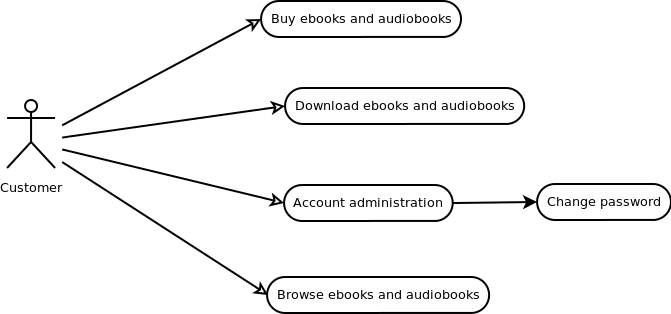
\includegraphics[scale=0.7]{Casemodel.png}
\caption{A use-case diagram describing the use cases of the Application.}
\label{casemodel}
\end{figure}

\subsection{Usecases}

\begin{enumerate}
\item 
Title: Logging in\\
Entry condition: The user presses the log in button.\\
Main Success Scenario:\\
  Step 1: Then the user enters his/her username and password.\\
  Step 2: He/she then submits the information by pressing a button.\\
  Step 3: His/her books are now loaded to the application, as paths to the locally downloaded book.\\
Exit condition: The login is successful.\\
Extensions:\\
  Extension 2a: The user writes a wrong username and/or password.\\
  Extension 3a: There is no internet connection.\\
\item 
Title: Buying book\\
Entry Condition: The user presses the buy button, figure \ref{Book information}.\\
Main Success Scenario:\\
  Step 1: The user enters his/her credit card details.\\
  Step 2: He/she then submits the information by pressing a button.\\
  Step 3: The book is added to the users account.\\
Exit Condition: The book is successfully added to the user account, the book information side, figure \ref{Book information} will now show a download button instead of the purchase button.\\  
Extensions:\\
  Extension 2a: The user writes wrong card details.\\
  Extension 3a: There is no internet connection.\\
  Extension 3b: The transaction was denied.\\
\item 
Title: Search for a book\\
Entry Condition: The user presses the search bar.\\
Main Success Scenario:\\
  Step 1: A search query is written.\\
  Step 2: The query is committed.\\
  Step 3: The results are shown.\\
  Exit Condition: A book is chosen.\\
Extensions:\\
  Extension 3a: There is no internet connection.\\
  Extension 4a: The query returned no books.\\
\end{enumerate}
\subsection{Class diagram}
The class diagram shown in figure \ref{uml}, describes the outline of the solution-domain. This design is evolving with the project as new challenges arise. The current challenges that resulted in this solution domain are described in depth in section \ref{sec:Syssum}.
\begin{figure}[H]
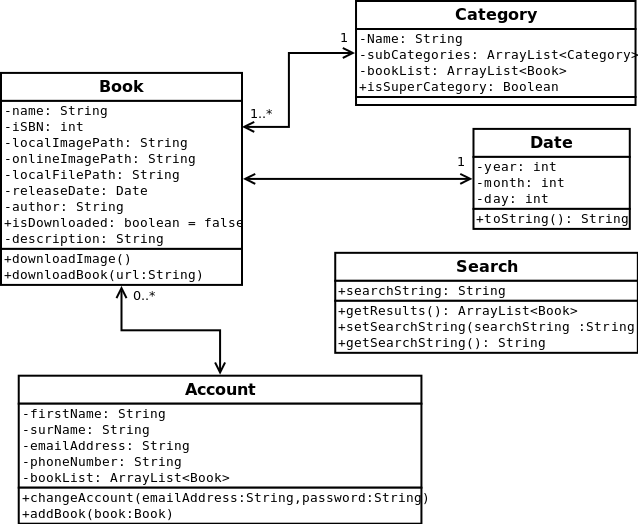
\includegraphics[scale=0.6]{uml.png}
\caption{A uml diagram over the Application}
\label{uml}
\end{figure}
\subsection{Sequence diagrams}

The sequence diagram shown in figure \ref{SeqDiaLogin} shows the chain of inner workings that is executed when the user tries to log in.
\begin{figure}[H]
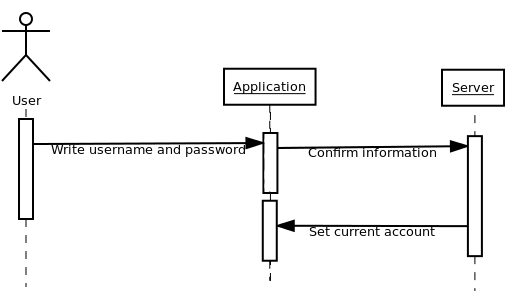
\includegraphics[scale=0.6]{SequenceDiagramLogin.png}
\caption{A sequence diagram for when a user logs in}
\label{SeqDiaLogin}
\end{figure}

The sequence diagram shown in figure \ref{SeqDiaBuyBook} shows the chain of inner workings that is executed when the user tries to buy a book.
\begin{figure}[H]
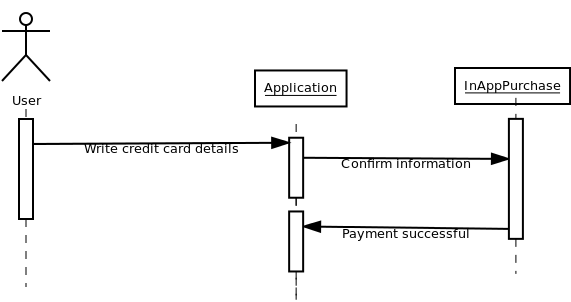
\includegraphics[scale=0.6]{SequenceDiagramBuyBook.png}
\caption{A sequence diagram for when a user buys a book}
\label{SeqDiaBuyBook}
\end{figure}

The sequence diagram shown in figure \ref{SeqDiaBookSearch} shows the chain inner workings that is executed when the user tries to search for books.
\begin{figure}[H]
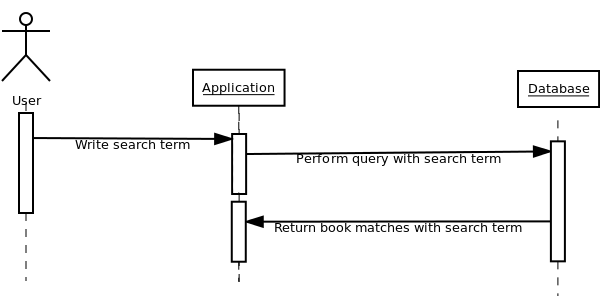
\includegraphics[scale=0.6]{SequenceDiagramBookSearch.png}
\caption{A sequence diagram for when a user searches for a book}
\label{SeqDiaBookSearch}
\end{figure}

\section{Systemdesign summary}
\label{sec:Syssum}
As of right now, we have developed a prototype of the application. What we need to do, is:\\

Database interaction through java:\\
The queries that the user makes regarding bought books and browsing for new books needs to be taken care of, the implementation of this depends on the WebAPI.\\
\\
A payment solution:\\
When a customer wants to buy a book, the system for handling this is needed. The Android SDK provides a tool for this, but it has yet to be implemented and fully understood.\\
\\
We also need a contract with a reader application as well as designing a login page when the application is launched.
\\\\
\begin{figure}
 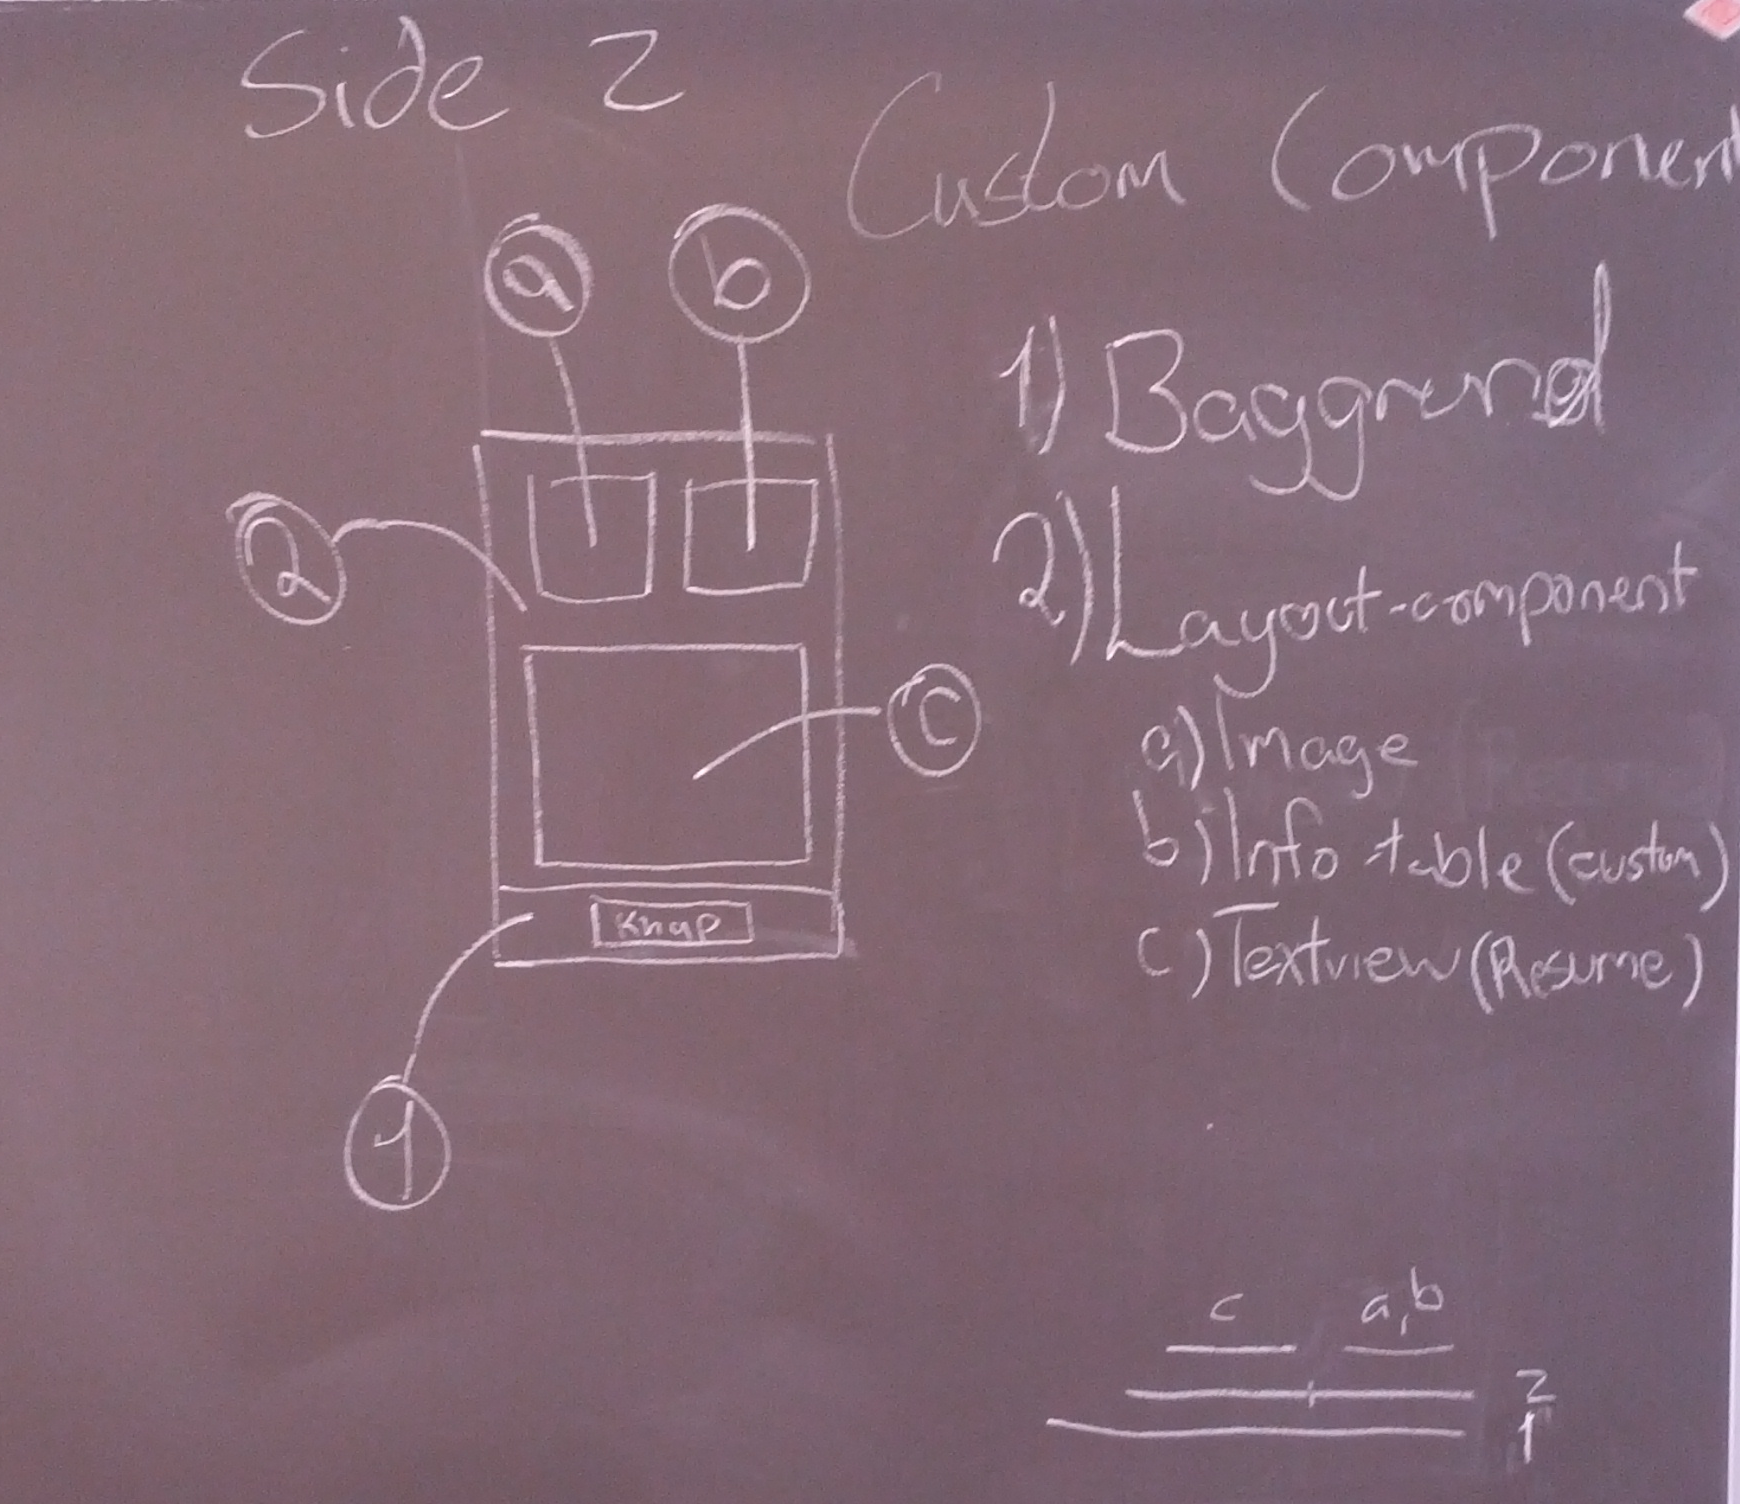
\includegraphics[scale=0.2]{Tavle}
\caption{Design of the activity, SpecificBook}
\label{Table0}
\end{figure}
\begin{figure}
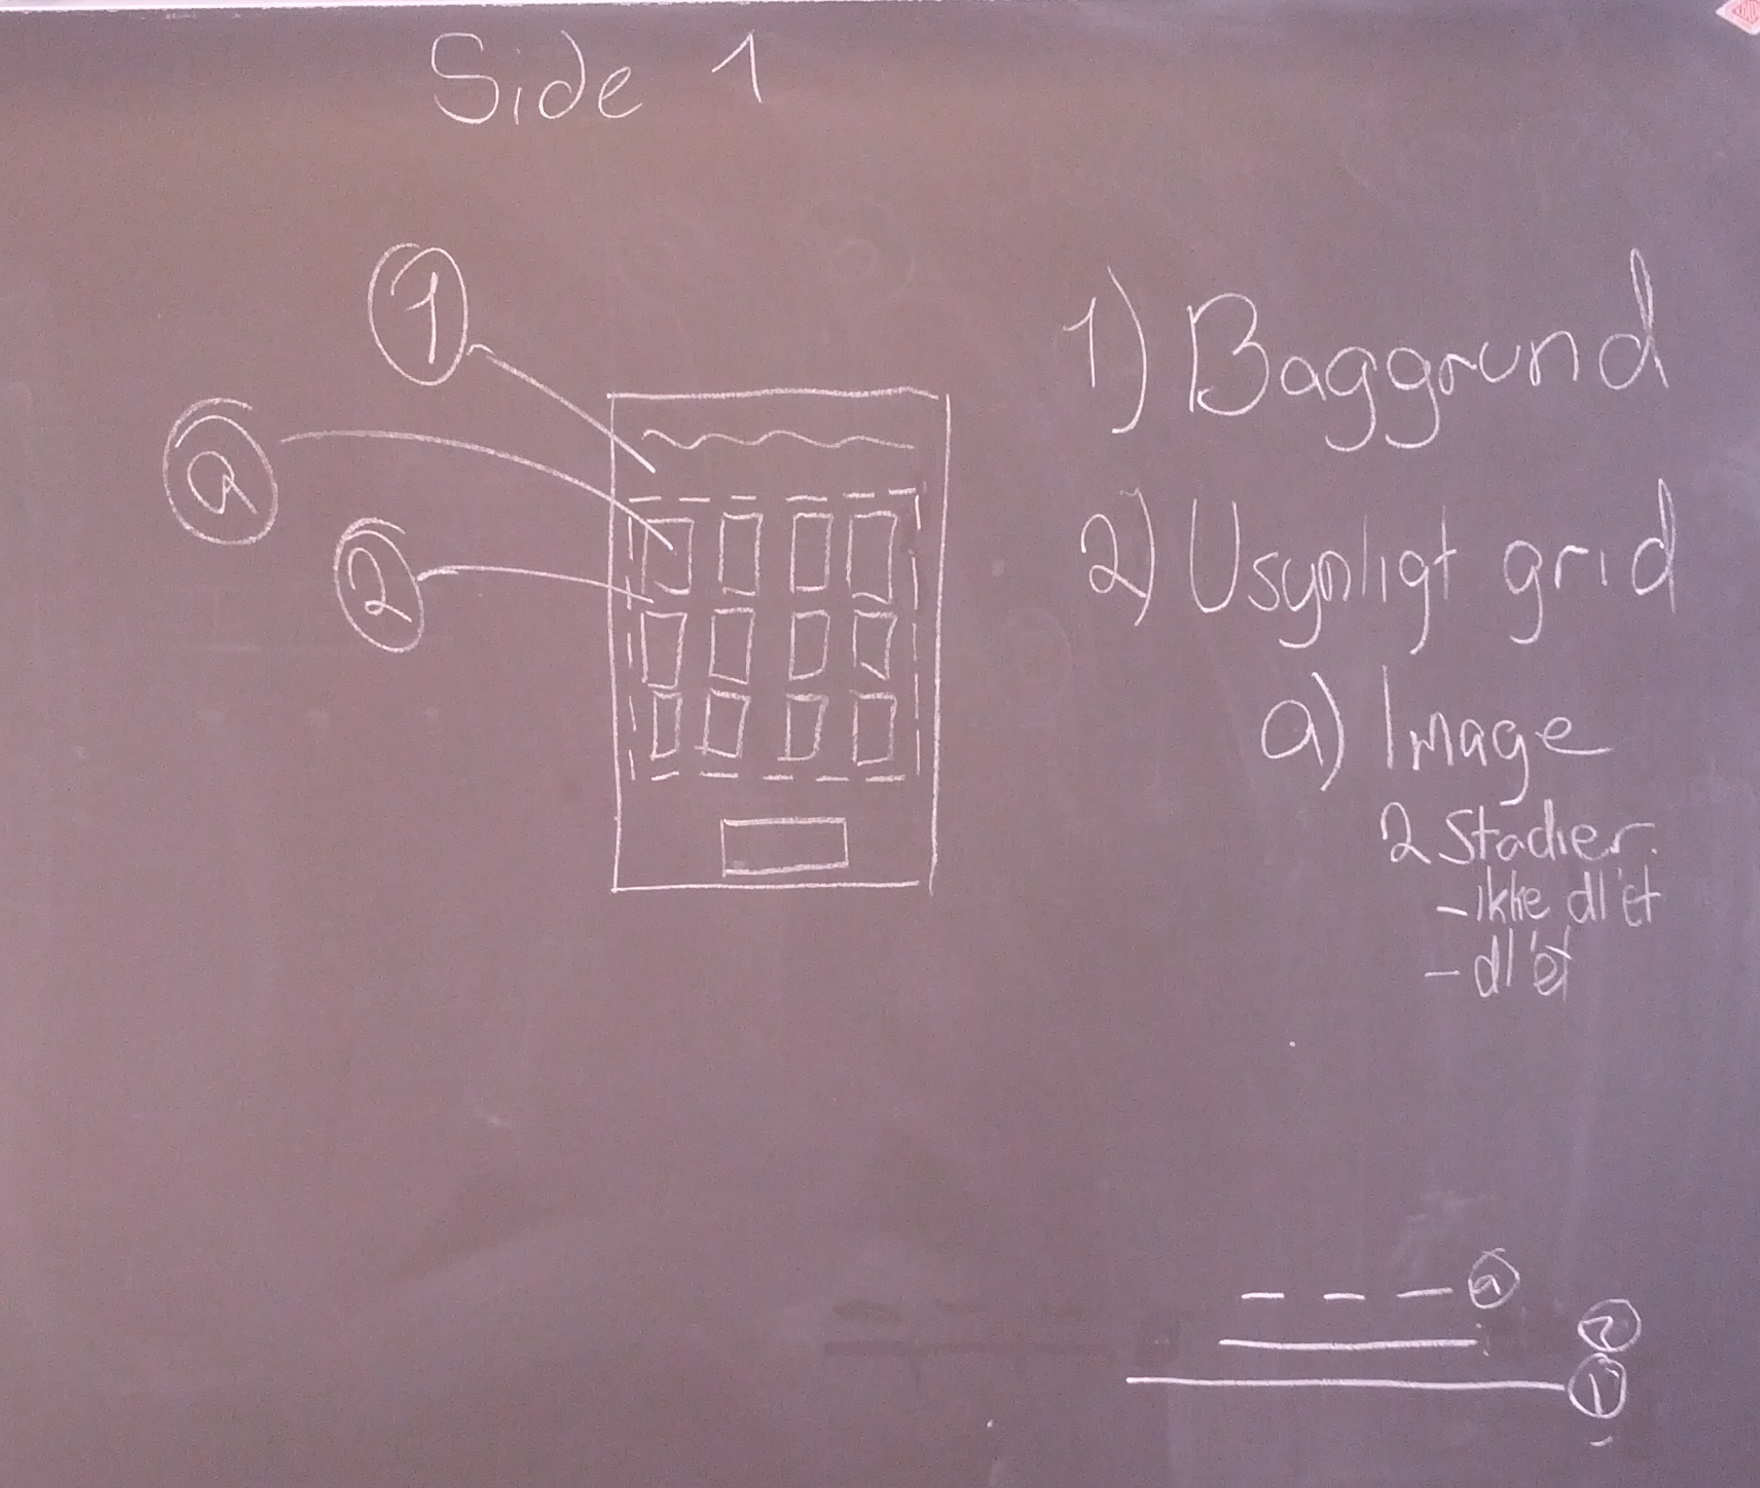
\includegraphics[scale=0.2]{Tavle1}
\caption{Design of the activity, YourBooks}
\label{Table1}
\end{figure}
\newpage
\section{Program- and systemtest}

Our testing regime has involved emulating the lowest level API we are developing for and executing the application directly on our android smartphones, which uses the highest available API level. Furthermore, each incrementation has been loaded up in different screens sizes, to test that the layout scales correctly. However, this testing regime does not apply to our prototype as it is developed to showcase our progress. Finally, testing has involved black-box testing as described in the following subsection.

\subsection{Black-box testing}
Since the last sprint, we have been performing black-box testing as soon as the individual sites were up and running, to examine the functionality of the applications current solution. Since the pages, as of now, do not consist of the most advanced code, the minor bugs found, has been solveable. This does not include the graphic layout.
\section{Userinterface and interaction design}
The external interfaces are here understood as the finished product GUI as it follows in Figure \ref{Front page},\ref{Book information},\ref{Categories} and \ref{Results}. The application GUI for the login page is yet to be designed.
\begin{SCfigure}
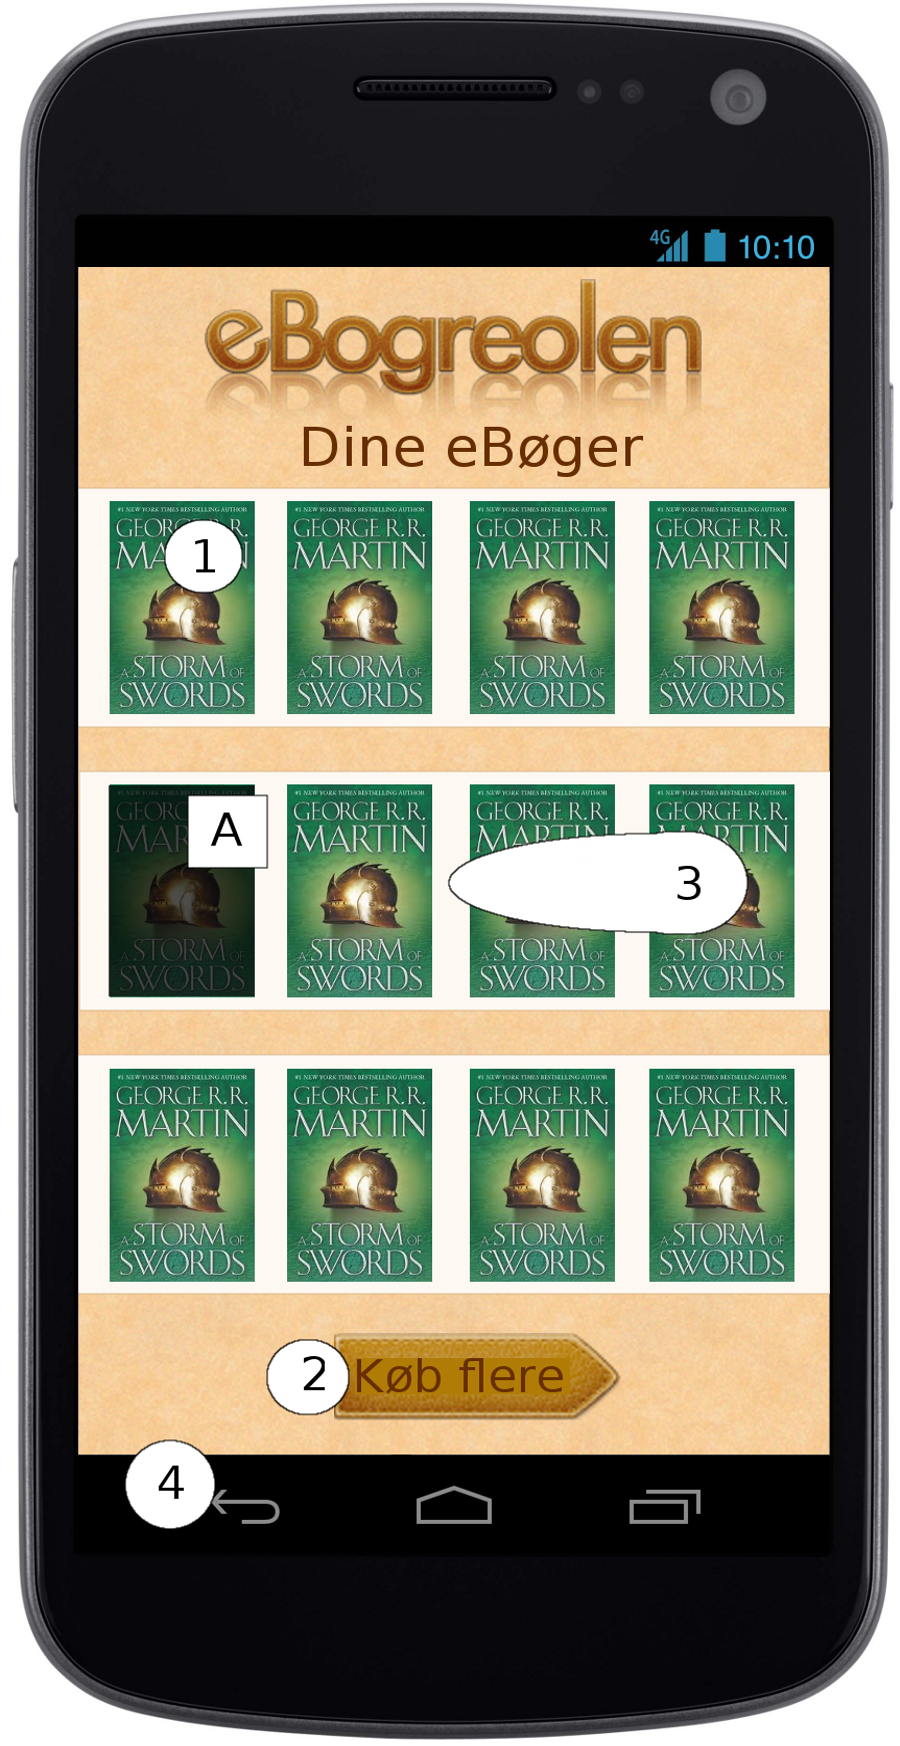
\includegraphics[scale=0.7]{gnexforside.png}
\caption{
\\
1. Open a page containing the information of a purchased book. This will lead to Figure \ref{Book information}.\\\\
2. Search/browse after more books to purchase. This will lead to Figure \ref{Categories}.\\\\
3. Swipe to the side to look at more of your books.\\\\
4. This button will always go one page back. If there are no more pages to go back to, the application will be closed.\\\\\\
A. This book is darkened, because the book has been purchased, but not downloaded.
}
\label{Front page}
\end{SCfigure}

\begin{SCfigure}
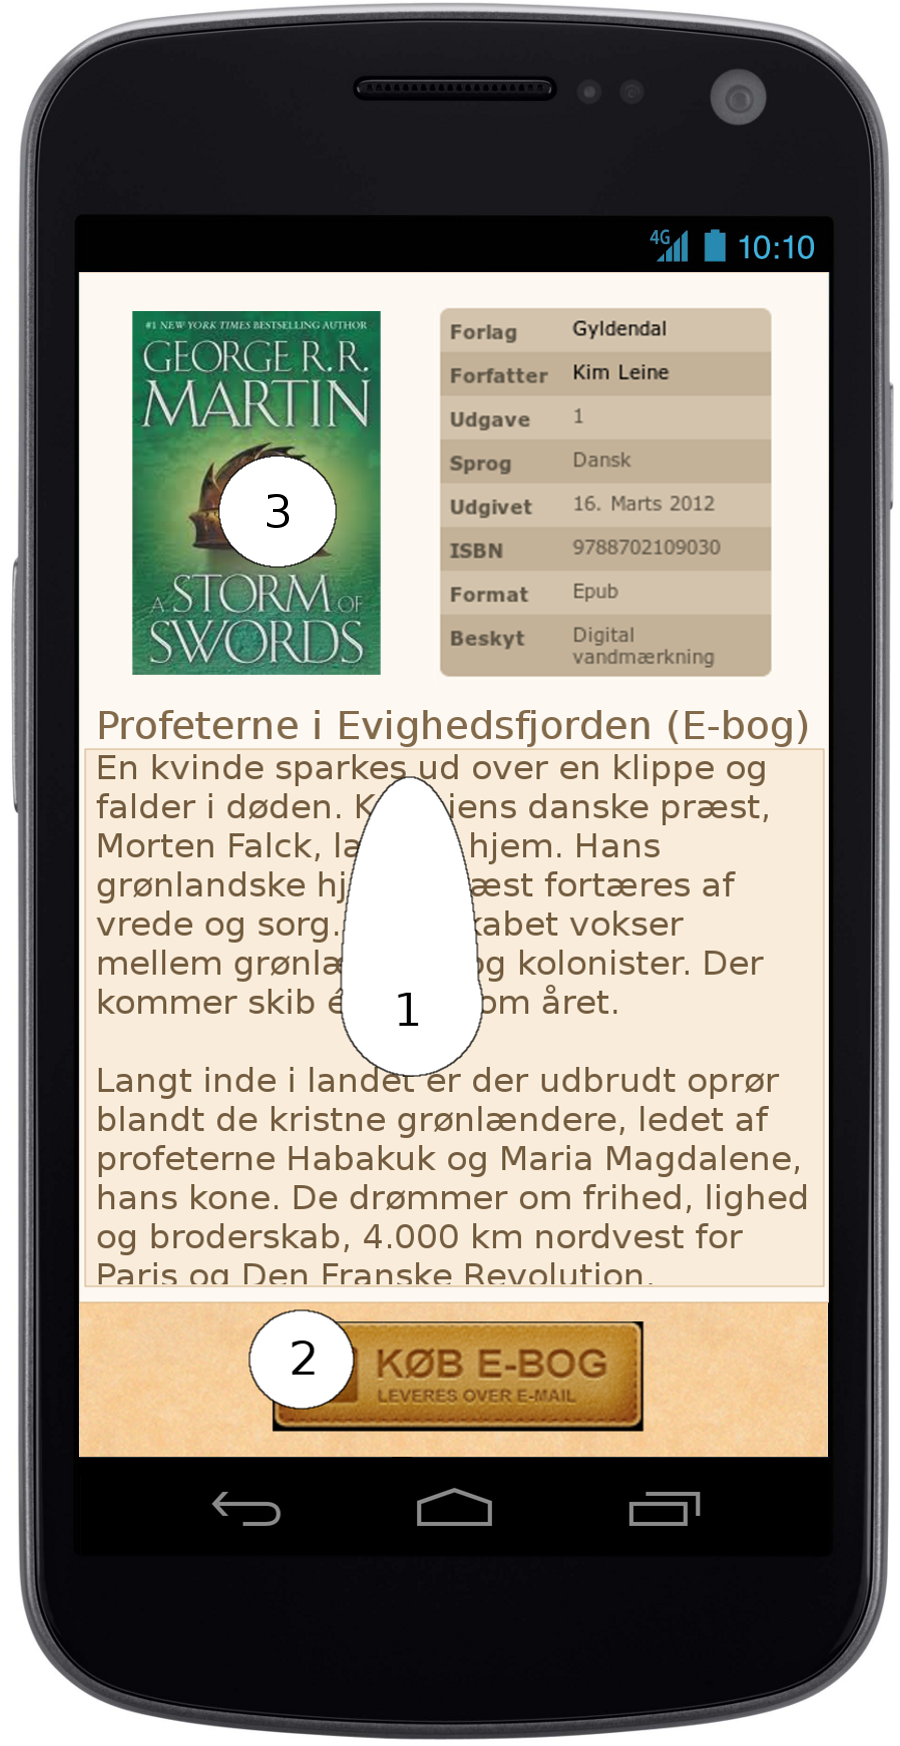
\includegraphics[scale=0.7]{gnexinfodownloadogkoeb.png}
\caption{
\\
1. Swipe up and down to read a description of the book.\\\\
2. This button can be a: Buy, Download, Read or Listen button, this depends on whether or not you own the material and/or if it is an audiobook or ebook.\\\\
3. Tapping the image enlarges it to a full screen view, tapping the image while enlarged will return to the displayed page.
}
\label{Book information}
\end{SCfigure}
\begin{SCfigure}
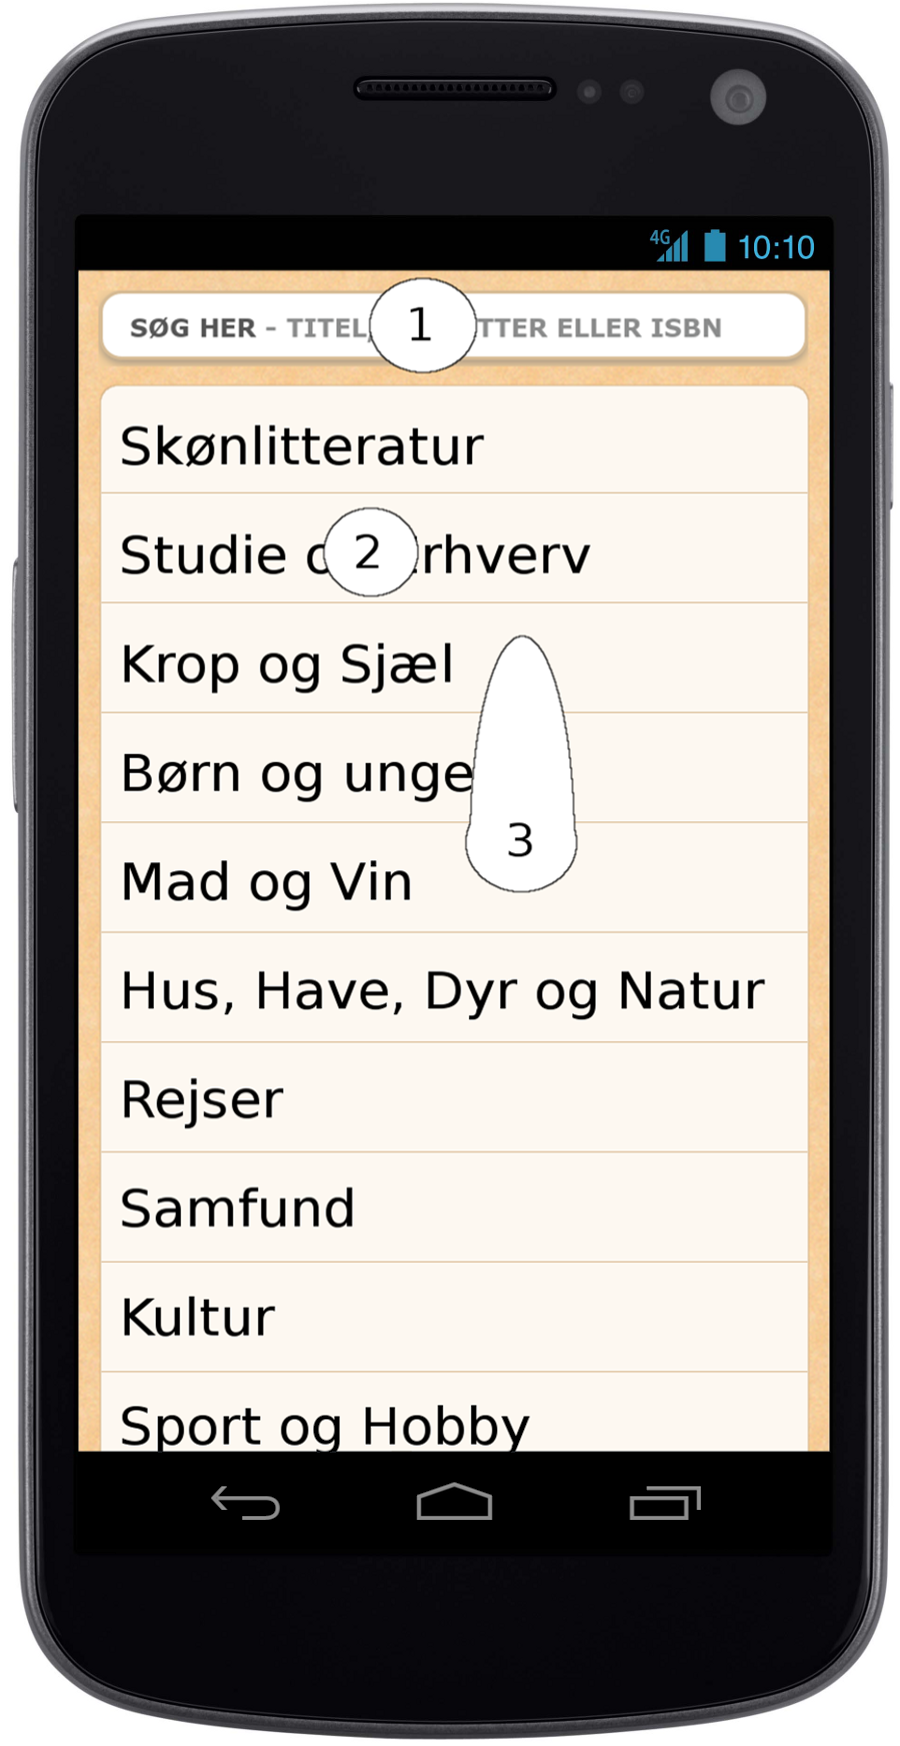
\includegraphics[scale=0.7]{gnexsoegeogbrowse.png}
\caption{
\\
1. This will access the search function, when a search is complete it will direct you to Figure \ref{Results}\\\\
2. This will open the category in this interface if it is a super category, and go to Figure \ref{Results} it is a sub category.\\\\
3. Swipe up and down to browse the categories.
}
\label{Categories}
\end{SCfigure}

\begin{SCfigure}
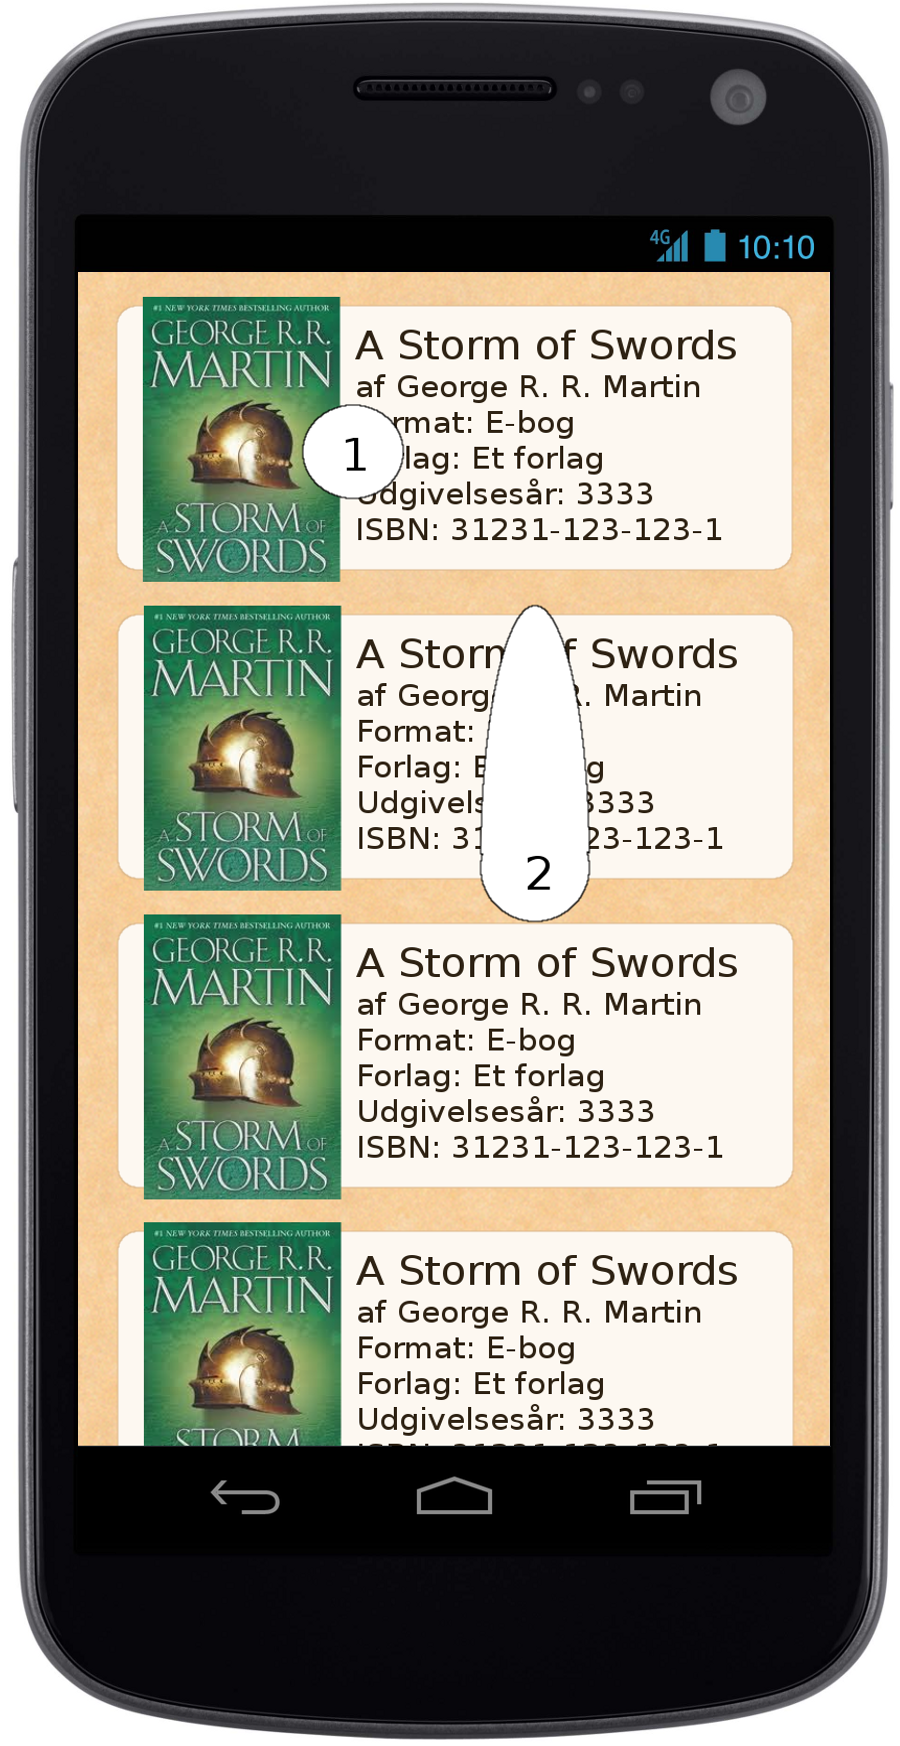
\includegraphics[scale=0.7]{gnexresultater.png}
\caption{
\\
1. This will take you to the information of the given book, this will lead to Figure \ref{Book information}.\\\\
2. Swipe up and down to browse the results.
}
\label{Results}
\end{SCfigure}

\subsection{Audio-visual presentation}
We now have a interactive prototype, with some dummy functionality. A presentation of the prototype can be found here: http://www.youtube.com/watch?v=WopMZ3KZ7Zc.

\subsection{Latest think-out-loud results}
The latest think-out-loud test was with a student who was asked to perform two tasks. Find a book called Storm of the Sword, then find the same book using a search, then purchase it and download the book to the device. The test was a pen and paper test using the activities figure \ref{Book information}, \ref{Categories}, \ref{Front page} and \ref{Results}, without comments. The student was confused about the results page, \ref{Results}, but after explaining that this page would contain all the books fitting to the chosen category, he was appeased. The rest of the first task went smoothly. When asked to search for the book, the student identified the search bar fast on the categories
activity, \ref{Categories}. The student found it annoying that in order to purchase the book and download the book, he had to return to the same pages twice when being send back after doing the purchase.
\section{Version Control}

Since the last commit, we have successfully merged together the GUIs described in Figure \ref{Book information}, \ref{Categories} and \ref{Results} and in the previous papers "Version control" section.\\
The classes from the first commits are still merged together with the rest, although unused, we still do not know if they will come in handy. With the new content added, we are now able to navigate between pages, due to the increased functionality.\\ 
Since the current version still is in the prototype state, it only contains dummy data for test purposes. A clone of the repository yields the code for an application that can be run on any Android device of version 2.3 or higher, though a path for a local ADK must be provided and some other system specific settings. Furthermore it will hold the most updated working application.\\

Se our complete commitlog at section \ref{Commit-log}
\section{Project collaboration}

Our group met several times during the last month for coding sessions. We've been working with linking different activities, so as to make the application interactive. The front-end is mostly done with the exception of a couple of surprisingly difficult custom views. \\
We've done no work individually during this iteration. We tried to assign specific jobs to individuals during the last iteration, but it was not very successful. We concluded that this was a result of learning the Java android SDK environment while developing, was much easier when we were sitting together.\\ 
This whole integration of the Java and XML code, to create a working and functional GUI, have generally shown to be a much more complex task than first anticipated, which has resulted in none of our functional requirement being met. The group has strong intentions of continuing to work with EBogreolen, in order to develop a complete application.\\

As for the communication with the client, we have recently had a meeting with eBogreolens in house developer Anders Hyldig about the functionality of the WebAPI he developed for us. We have through this gained a working understanding of the WebAPI, though we are still struggling with implementing it in our android project. As a result of this we have not been able to implement it in our current prototype.\\
This could have been avoided, by learning how to implement it while we waited for it to be developed, instead of postponing it until it was available.\\ 

We have developed scoreboard as a motivational tool, which entitles the person in lead to small benefits (bragging rights, beers etc.). This has benefited the group immensely as we all thrive in a competitive environment. Our scoreboard uses 'experience' points, gained through working with the project and completing tasks associated with our sprint backlog. These experience points are distributed to the group participants by a point generator, found here: \url{http://www.VixQIT/XP/XP.php}, that generates a random amount of points in a certain range around x. Tasks are worth points equal to the hours of work estimated during our scrum and these translates into points that provides the range from your random gain of experience. The experience needed to level up increases each time following the Fibonacci sequence.\\
\\

\newpage
\section{Review: M.A.D experience}
\label{Review1}
The article reflects on the experience of developing a Global Customer Service System (GCSS) for a Danish shipping company, presumably Maersk. The developers of the GCSS have no experience with the reality of commercial shipping, and the challenges that follows. The developers experience can be classified as: the ethnographer, the participatory designer and the Object Orientated developer.

The article discusses at length the MAD project from the perspective of the three classifications of expertise. The domains they each work within has given rise to the need of some common understandings of particular problem instances. A great example of this is the re-routing problem named the Bremerhaven instance.

The idea of defining an instance of common issues identified within the client as a benchmark for communication within the working group, as well as an early test, is brilliant. That the team was able to identify an instance that they could expand upon to use throughout the project, is probably a consequence of highly skilled and seasoned individuals on the team, hence not something that we can do yet. Defining such instances would definitely be of benefit to the group in future projects.

Just as in the book, the article puts much emphasis on the value of testing and working with the client. As with the developer group has assigned a specific sub group that is working with the test. The book writes on the subject "subsystem teams can double as a testing team for components developed by other subsystem teams".  
\newpage
\section{Programming as Theory Building}
\label{Review2}
The article argues from the basis that any program can not only be designed and produced, but must also cater to changing environments and as such the primary aim of programming is not writing the program, but for the programmer to develop a theory which solves the problems through program execution.\\

The theory to be built by the programmer must be such that "the programmer having the theory of the program can explain how the solution relates to the affairs of the world that it handles". The programmer should be able to explain why each part of the program is written as it is, hence justifying all decisions for the program text. Lastly a programmer that has developed a theory for a program is able to respond to any call for modification constructively.\\

Our group is very fond of this idea, finding that often the best way to learn and understand new languages is through the guidance of a more seasoned computer scientist. Learning from books and documentation often leads to misinterpretations, that can require hours of backtracking to rectify. Hours, that can often be saved by explaining once there is an error pointed out by the more skilled programmer.

The book identifies modifiability as a design goal. They defines this as the ease of which a modification can be done to the developed software. The article comments on modifiability as something that can only be done successfully while the program is still alive. 
\newpage 
\section{Appendix}
\subsection{Commit-log}
\label{Commit-log}
The following is the commitlog for our repository at https://github.com/VixQIT/EBogreolen where our code is accessible as well:
\begin{verbatim}
$ git log --pretty=oneline
0a92c56627e8547191f98ae61c434542ceb4f94a update
cd59b794a7614691b691fcf1fddb5034d6eeaf7e update
81f96c3c2b2cf33ceaabfdf0b63c3ddb8d547d6b Test
d5421935758de876b9b613cacec4167c3f2208e6 Test
fa79e32927f67ccc7483277525a7f0b4a855405d minor changes
fae66c3414c4de7a8f8f17b1118e982920fe5a94 minor changes
5779ac9da57787a03d2baa48a8188b66204b3e23 Fixed various items
99a72ad7cedfda5019cba6f3801334ee5481204e SpecificBook update
12de19605b065b312fb9937fab08b6d8bc4374a0 Bookinfo setup
4e7388ef4cecb299efb3d91ffbf4bf95f4d3ab0f Connected SearchActivity and Results
5a00d025e589d6f6e9fa79ecbf11de3ed88cf5ba SearchActivity changed
e5f1f6f6a8f3a8165ab612f0cc64fdc74c3a942c minor design tweak
415efdf381a0588cde453baf74cc5ab30c4c655a Added result activity - working
d65d0d1d501d93c00f3e0bc3fce76bdebdfd67f2 Added result activity - working
6bd44dbbae9fe9b26f815565acf2b13a66730bff Added listener to an ExpandListChild, a
fefa828bf15b9834e0998599c5416452ab70bfea bin/EBogreolen
9b2a7766b65fac09eddf2f4307265afa1734558f Layout changed in search_activity
f94a3c72fa3e965884fa84fd1fe995bb67e266e7 minor changes
7d66bd221d9605a95252307425428e191c5aa967 minor changes
7d76ce7922967e420a688e1605d6e948305e97a5 results slide update
f61f9af4aa0710510934c087e9f970ad2b10797c ingenting
60b87c7f992e1c99b919d117d5778466af3f14d5 Minor features changed
d59dce2ad2165e732f8167cde990ab03f9bdc8c5 Locked screen orientation of SearchActi
b80bd05310576fc275b51b98ada6a5c93c1db50b Added portrait mode to YourBook
cd08044f313ef9846fb9a189e7e031b59e84a64f Added portrait mode to YourBooks
1a47e565ef07a0c8771d6ef07fe98fbe1b648cd7 Button functionality
33270a15351cb5d74a06694068066b436a5bd36f Merged together with the SearchActivity
a38eadd6db8d30e7af74551e70fe71247be70018 Merged together with the SearchActivity
0dd7a7751efa1eab53e6ec04d769cad52439e289 added Results activity
cb721602919bbc65f034ff386ed1fb89ff8b6f99 Updated YourBooks to add books programa
840c6cbdac85855d816f3f55c7c036488462f671 added application
05dcec5b8ada987372b125ca26a0989dcf74de75 added application
3f7efb800accf646de7f0eb041e987341e7b8191 Test
064f99889deda672a1362a13fc4e1960bb002785 Cleaned the project
9dd6bad8eec27a1012dcf399187a98ad42de842d Fix of your books activity
96927130e41cf1f71b08aea0578cd424b3c0c9a7 Setup of android app environment, and a
258566b216827dd09a6186042069f4ecb563faf5 Merge branch 'master' of https://github
5176586754383ad696ecc8da6e3b1a089b611ad1 First commit
86bf9e9a7090a87a986ecf6bf7ec34ed094a56f7 Initial commit
\end{verbatim}

\end{document}